


\documentclass[runningheads,a4paper]{llncs}

\usepackage{graphicx}
\graphicspath{ {images/} }
\usepackage{amssymb}
\setcounter{tocdepth}{3}
\usepackage{graphicx}

\usepackage{url}
\usepackage{blindtext}

\usepackage[utf8]{inputenc}
\usepackage[T1]{fontenc}
 
\newcommand{\keywords}[1]{\par\addvspace\baselineskip
\noindent\keywordname\enspace\ignorespaces#1}

\begin{document}

\mainmatter  
\title{2º Projecto de PLOG}

\author{Nuno Freitas e Daniel Garrido} %


\institute{Faculdade de Engenharia da Universidade do Porto\\ Rua Roberto Frias, sn, 4200-465 Poto, Portugal
}


\maketitle

\section{Introduction}

Este projecto foi feito no âmbito da disciplina de “Programação em Lógica” e teve como objectivo a construção de um programa em Programação em Lógica com restrições.\\ 
	Foi permitido aos estudantes da cadeira escolher de uma seleção de Problemas de Otimização e de Decisão e o nosso grupo decidiu escolher o puzzle 2D “Tents”.\\ 
	O resto de este artigo vai seguir a seguinte estrutura:\\

\begin{enumerate}  
\item Descrição do Problema - Nesta secção vai ser descrito em detalhe  o problema de decisão que é o puzzle “Tents”.
\item Abordagem - Nesta divisão do artigo vai ser explicado a modelação do problema como um Problema de Satisfação de Restrições a partir das 4 subseções seguintes
\item Abordagem
\begin{enumerate}
\item  Variáveis de descrição - Esta subsecção tem como objectivo explicar as variáveis                      de decisão e os seus domínios.
\item Restrições - Serão aqui descritas as restrições rígidas e flexíveis do problema e a sua implementação utilizando o SICSTUS Prolog.
\item Descrição da estratégia de etiquetagem implementada.
\end{enumerate}
\item Visualização da Solução - Explicação dos predicados que permitem a solução em modo de texto.
\item Resultados
\item Conclusão
\end{enumerate}


\section{Descrição do problema}
O puzzle Tents consiste em colocar tendas num tabuleiro onde existem árvores previamente colocadas. As tendas têm de ser colocadas horizontal ou verticalmente ao lado de uma árvore. As tendas não podem tocar nas outras tendas, nem mesmo diagonalmente, e para cada árvore no tabuleiro tem de existir uma tenda. \\
Os números que se encontram junto ao tabuleiro indicam o número total de tendas que podem existir nessa coluna/linha.\\


\section{Abordagem}

\subsection{Variáveis de Descrição}

A solução vai tomar a  forma de uma lista simples  de tamanho igual ao tabuleiro dado por S*S sendo que S vem retirado de size(S), uma função que vem com a definição do tabuleiro.\\
	Para definir a solução final e aplicar correctamente as restrições na definição do tabuleiro são criadas as funções tree(A,B),  column(A,B) e row(A,B) que respectivamente designam o espaço onde vão estar as árvores às quais as tendas vão ter de estar juntas adjacentementem, delimitam o número de tendas (B) existentes nessa coluna(A) ou linha dependo do uso de column ou row.\\
	O domínio da solução é definido  pela dimensão do tabuleiro tal e qual como a solução.




\subsection{Restrições}

Apesar do Tents ser um puzzle simples, foi necessário implementar varias restrições para chegar aos resultados esperados. Essas restrições foram:\\

1 - O número de árvores e de tendas tem de ser igual. 
Cada árvore tem de ter uma e só uma tenda associada. Para tal verifica-se que a soma dos elementos da lista solução é igual ao número de árvores no tabuleiro.\\

2 - O número de tendas à volta de uma árvore tem de ser maior que zero.
Como cada árvore tem de ter uma tenda à sua beira (horizontal ou verticalmente), verifica-se que a soma das posições (horizontal ou verticalmente) validas a volta da árvore tem de ser maior que zero.\\

3 - A número de tendas numa linha/coluna tem de ser igual ao número indicado
Para verificar que cada linha/coluna tem o número de tendas suposto, somam-se os elementos de cada linha e cada coluna individualmente e verifica-se que tem de ser igual ao valor indicado pelo puzzle.\\

4 - Cada quadrado 2x2 do tabuleiro tem de ter um número de tendas menor que 2
Uma tenda não pode tocar noutra tenda, nem mesmo diagonalmente. Para assegurar esta restrição, somam-se os elementos a este, sul e sudeste de cada célula da linha de 1 a S – 1 (coordenada X), de todas as linhas de 1 a S – 1 (coordenada Y). Esta soma tem de ser menor que 2.\\



5 - Duas árvores não podem ter associada a mesma tenda
Como tem de haver uma tenda para cada árvore, duas árvores não podem partilhar a mesma tenda, situação que pode acontecer quando uma árvore tem outra árvore junto dela diagonalmente, ou a uma distancia de duas células na horizontal/vertical. Para assegurar que esta situação não acontece encontram-se todos os pares de árvores que se encontram nesta situação e verificamos que a soma das células a volta das duas árvores volta na horizontal e vertical tem de ser maior que 1.\\

6 - As posições ocupadas pelas árvores não podem ser tendas.
Para assegurar que nenhuma tenda é posicionada no lugar de uma árvore, restringe-se que cada posição ocupada por uma árvore tem de ser igual a 0.\\


\subsubsection{Descrição da estratégia de etiquetagem implementada}

Para este puzzle não foi necessário utilizar uma estratégia de pesquisa, visto que é suposto haver uma única solução para cada puzzle.

\section{Visualização da solução}

Para ser possível visualizar o resultado são impressos dois tabuleiros na consola, um com apenas as árvores e as pistas e outro com as tendas, árvores e pistas. Na representação escolhida, um 'T' representa uma árvore e o conjunto de caracteres '/|\' representa uma tenda. 
Os números no lado direito e em baixo representam o número de tendas que essa coluna/linha tem de ter.

\begin{figure}
  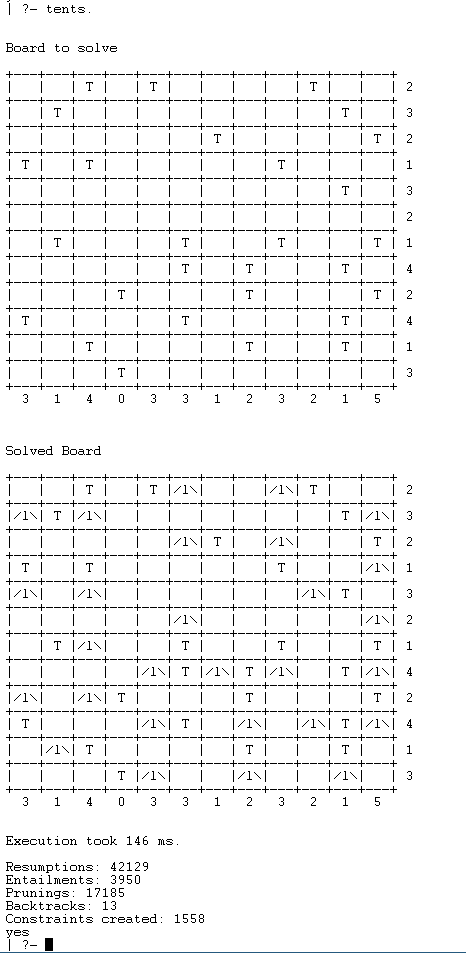
\includegraphics[scale=0.8]{images/result.png}
  \caption{Resultado obtido na consola ao correr o programa no SICStus.}
  \label{fig:Resultados}
\end{figure}

\subsection{Resultados}

Os resultados obtidos são suficientemente conclusivos e somos capazes de retira as seguintes coclusões:\\

Tamanhos abaixo de 7x7 são extremamente rápidos e a partir de 12x12 passam a ser mais lentos
Quanto maior o número de colunas e linhas maior o tempo de processamento se a diferença entre o número de linhas e colunas não for demasiado extremos.\\


Size 7x7\\
9 trees, 7cosl, 7 rows - 13s\\
9 trees 3 cols 7 rows  9ms\\
9 trees 7 cols 4 rows 11 ms\\

Size 6x6\\
8 trees, 2 cols, 2 rows - 12 s\\

Size 12x12 \\
28 trees, 12 cols 12 rows - 479 ms\\
28 trees 6 cols 12 rows - 256 ms\\
28 trees 12 cols 6 rows - 423 ms\\
28 trees 6 cols 6 rows - 311 ms\\
28 trees 10 cols 3 rows - 632 ms\\


\section{Conclusão}


Concluido este projecto, o nosso grupo pode concluir que em determinadas situações o uso de Prolog com restrições é extremamente útil. A partir de este tipo de programação é facilitado o desenvolvimento de programas complexos.\\
	O programa foi concluído com sucesso visto que para uma board válida o programa encontra com eficiência a solução única. \\
	No entanto o projecto podia ser melhorado com a inclusão de geração de puzzles automática que não foi possivel implementar.\\

\end{document}
